\chapter{Planificación} \label{sec:planificacion}

\section{Metodología utilizada} \label{sec:metodologia}
Para el desarrollo del proyecto he elegido una \textbf{metodología ágil}, en concreto la metodología \textbf{kanban}.
Esta metodología es muy utilizada en la actualidad y consiste en unas prácticas que permiten un trabajo de entregas que se va incrementando para el desarrollo de un producto. \\\\
La gran característica de estas metodologías y por lo que reciben su nombre es su agilidad ya que consiste en presentar una serie de objetivos y/o requisitos necesarios que se van dividiendo en problemas más pequeños 
y se van resolviendo. A estos problemas se les asigna una prioridad y se asigna al personal que va a trabajar en el proyecto.\\\\
Otras características de esta metodología son que el cliente va a poder empezar a utilizar el producto porque se va a ir desarrollando y muy pronto va a tener un software funcional, 
además, permite la posibilidad de ir añadiendo nuevos problemas a resolver o adaptar los actuales a lo largo del desarrollo del proyecto y evita la documentación excesiva, dando mucha flexibilidad tanto al programador como al cliente.\\

Después se hace una planificación en la que se hace una estimación de los tiempos de entrega.
A partir de ahí estos requisitos que bien pueden ser historias de usuario, tareas de mantenimiento o corrección de bugs del proyecto se van realizando.
 
\newpage
\section{Seguimiento del desarrollo} \label{sec:seguimiento}

Para el seguimiento y gestión del desarrollo he utilizado el software de control de versiones
git \cite{git} en la plataforma Github \cite{Github}.\\\\
Esta plataforma me permite mediante un tablero organizar todo el proyecto
y tener un listado de requerimientos mediante historias de usuarios y tareas pendientes (issues) asignándoles
prioridad, asignándoselas a usuarios, aunque en este caso todas estarán asignadas a mí ya que es un proyecto personal 
y más posibilidades.\\\\
Además, para estar en contacto con mi tutor, he utilizado un Bot de Telegram que he conectado con mi repositorio y 
configurado para que cada commit, creación/cierre de issues o comentarios se notifiquen en un grupo de Telegram en el que estamos mi tutor y yo
junto con dicho Bot.\\

\section{Flujo de trabajo} \label{sec:flujo_trabajo}

El flujo de trabajo que he seguido para el desarrollo de proyecto ha sido el siguiente:\\\\

\subsection{Kanban}

Se ha creado un proyecto de Github y se ha utilizado un tablero Kanban para gestionar las historias de usuario y las issues del proyecto.\\

El Kanban del proyecto puede verse en el siguiente enlace:
\url{https://github.com/josemip98/TFG/projects/1}

\begin{figure}[H]
  	\centering
  	\noindent\makebox[\textwidth]{
	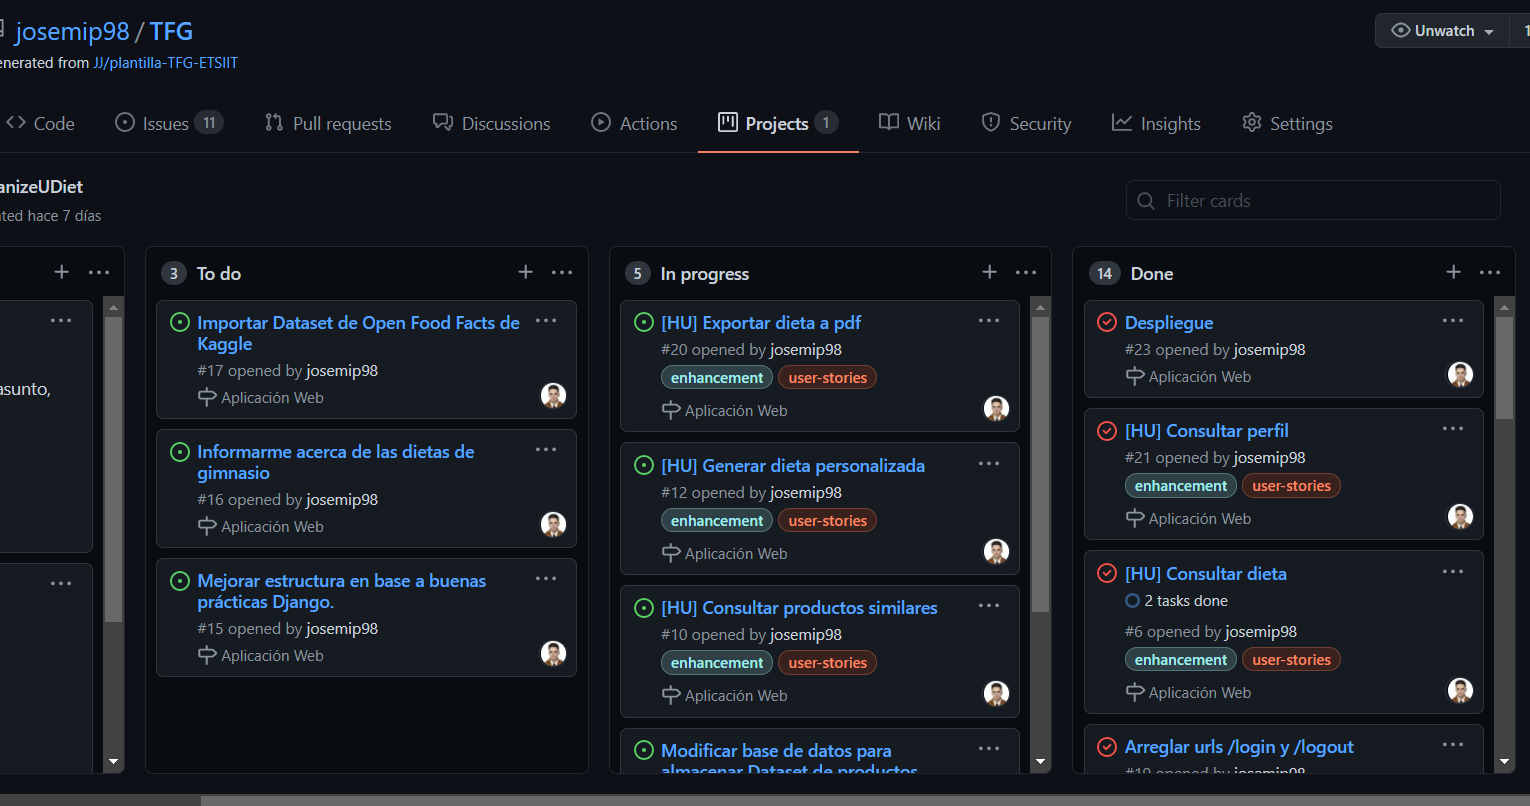
\includegraphics[scale=0.4]{kanban.png}}
  	\caption{Tabla Kanban del proyecto.}
	\end{figure}

\subsection{Historia de usuario}

Después se han creado todas las historias de usuario.
Se pueden encontrar todas las historias de usuario creadas en el anexo \ref{anexo} o en el repositorio de Github\cite{user-stories}.\\\\
Una historia de usuario es \textbf{una funcionalidad que el usuario o desarrollador espera}.
Además, podemos añadir tareas que necesitamos cumplir para completar la historia de usuario o detalles técnicos.
El modelo a seguir para la creación de historias de usuario es:
 
\textit{Como usuario/desarrollador quiero poder [funcionalidad] para [razón dicha funcionalidad].}

\begin{figure}[H]
	\centering
	\noindent\makebox[\textwidth]{
	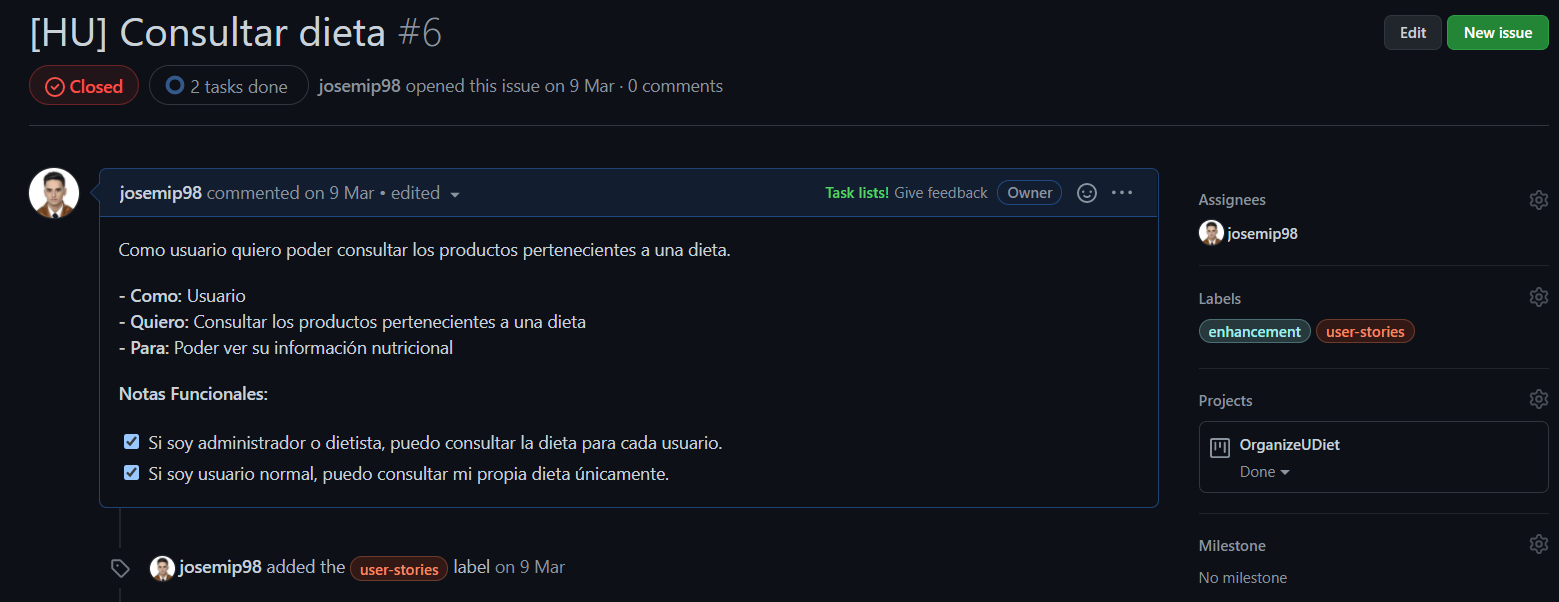
\includegraphics[scale=0.4]{hu.png}}
	\caption{Ejemplo historia de usuario.}
  	\end{figure}

\subsection{Issues}

Una vez creadas las historias de usuario las he dividido en tareas más pequeñas llamadas issues, 
además de añadir otras tareas que me hayan sido necesarias tanto para el desarrollo, como para el mantenimiento, 
documentación o corrección de bugs.\\
Se pueden encontrar todas las issues creadas en el repositorio de Github\cite{issues}.

\begin{figure}[H]
	\centering
	\noindent\makebox[\textwidth]{
	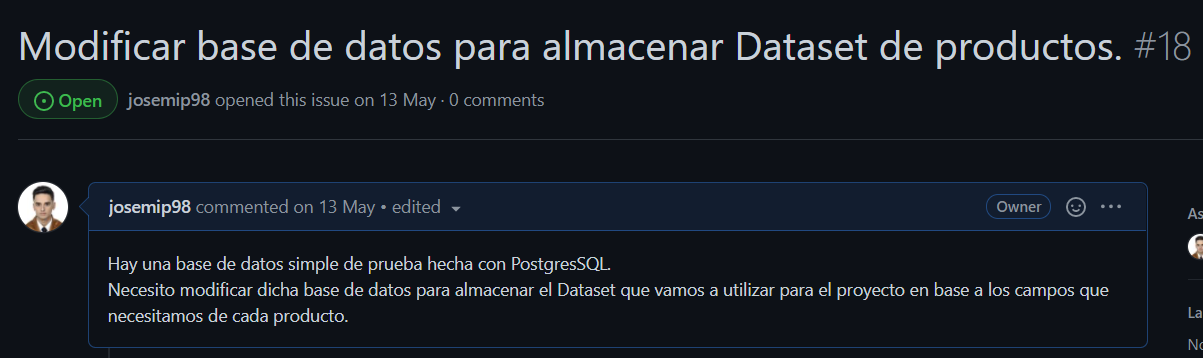
\includegraphics[scale=0.4]{issue.png}}
	\caption{Ejemplo de issue.}
  	\end{figure}


\newpage
\subsection{Etiquetas}

Por último, mencionar que se han utilizado las etiquetas como forma de categorizar las issues pendientes ya sea asignándoles prioridad o describiendo si es una issue de documentación, si es un bug, historia de usuario...
Además, podemos crear etiquetas a nuestro gusto según las necesidades que tengamos.

\begin{figure}[H]
	\centering
	\noindent\makebox[\textwidth]{
	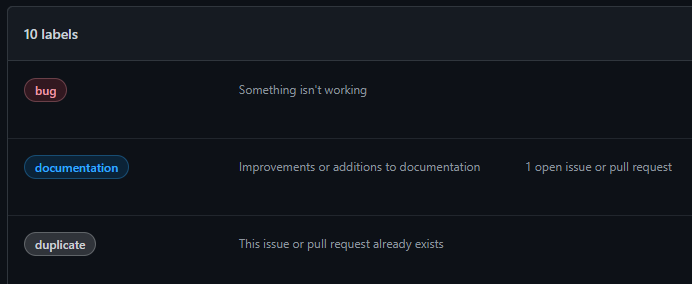
\includegraphics[scale=0.4]{etiquetas.png}}
	\caption{Ejemplo de etiquetas.}
	\end{figure}